
\section{Policy}
\label{fig:policy_description}

The policy dictates the agent's behaviour. The policy is responsible for selecting actions from observations. The policy is trained using the \ac{PPO} algorithm. The algorithm has proven to be very reliable \textcite{ppo}. The algorithm can be used for our continuous control task.

A \ac{NN} is used as for the policy here. The \ac{NN} belongs to the class of \acp{CNN}. This architecture was chosen since \ac{CNN}s are ideal for processing image data. The convolutional network's architecture follows the specifications from \textcite{human_level_control}. This architecture has been used successfully in comparable \ac{RL} control tasks.

The network takes the output of the observation preprocessing as input. This input is a three dimensional tensor, similar to an image. The network consists of convolutional and fully connected layers. The network produces two outputs, an action distribution and a value function. The action distribution is a probability distribution over the action space.
The value function is a scalar value that estimates the expected return of the current state. The value function is not used during the action inference. The value is only used during the training of the policy network. It is used to compute the advantage function which is required for the loss in \ac{PPO} \textcite{ppo}.

% value or is it the critic? --> it is value


% human_level_control definiert das NatureCNN welches wir nutzen um die features zu extrahieren
% human_level_control hat einfaches Q-learning verwendet, nicht PPO



\subsection{Observation Space}

The input space of the \ac{NN} is three dimensional. The input is structured like images with $width$, $heigth$ and $channel$ dimensions. The dimensions are determined by the agent's camera image dimensions, preprocessing parameters and the memory mechanism. The input space is a tensor with the following dimensions:

\begin{align*}
    width    & = \frac{agentImageWidth}{downsampling\_factor}  \\
    height   & = \frac{agentImageHeight}{downsampling\_factor} \\
    channels & = frame\_stacking \cdot num\_color\_channels
\end{align*}

The tensor values are integers in the range $[0,255]$. Storing the pixel intensities as integers saves a lot of memory compared to floats.


\subsection{Action Space}

The environment's action space is a two dimensional scalar, the dimensions are called $leftAcceleration$ and $rightAcceleration$. The values are restricted to the range $[-1,1]$, see \ref{fig:action_space}. They dictate the agent movement \ref{cha:agent_description}.


\begin{figure}[!h]
    \centering
    \begin{tikzpicture}[%
            every node/.style={
                    font=\scriptsize,
                    % Better alignment, see https://tex.stackexchange.com/questions/315075
                    text height=1ex,
                    text depth=.25ex,
                }, outer sep=auto
        ]

        % draw empty rectangle
        \node[fit={(0,0) (4,4)}, inner sep=0pt, draw=blue, thick] (space) {};
        \node[anchor = north east] at (0, 0) {-1, -1};
        \node[anchor = west] at (4, 0) {-1, 1};
        \node[anchor = south] at (0, 4) {1, -1};
        \node[anchor = west] at (4, 4) {1, 1};

        \node at (0,0)[circle,fill,inner sep=0.001pt]{};
        \node at (0,4)[circle,fill,inner sep=0.01pt]{};
        \node at (4,0)[circle,fill,inner sep=0.05pt]{};
        \node at (4,4)[circle,fill,inner sep=0.1pt]{};
        \node at (2,2)[circle,fill,inner sep=0.0pt]{};

        \node[anchor = north] at (2, 2) {0, 0};

        \draw[<->,thick] (0, -0.2) -- (4, -0.2);
        \node[anchor = north] at (2, -0.2) {rightAcceleration};

        \draw[<->,thick] (-0.2, 0) -- (-0.2, 4);
        \node[anchor = east] at (-0.2, 2) {leftAcceleration};

    \end{tikzpicture}
    \caption{the two-dimensional Action Space}
    \label{fig:action_space}
\end{figure}


\subsection{Architecture}
\label{sec:network_architecture}

The \ac{NN} produces two outputs, the action distribution and a value estimate. The outputs are produced by sections of the network called the action and value head. The action head produces the action distribution. The value head produces the estimate of the state's value. 

The action and value head share the first part of the \ac{NN}. They are built on top of the feature extractor. The full structure is shown in \ref{fig:network_structure}.


\begin{figure}[!h]
    \centering
    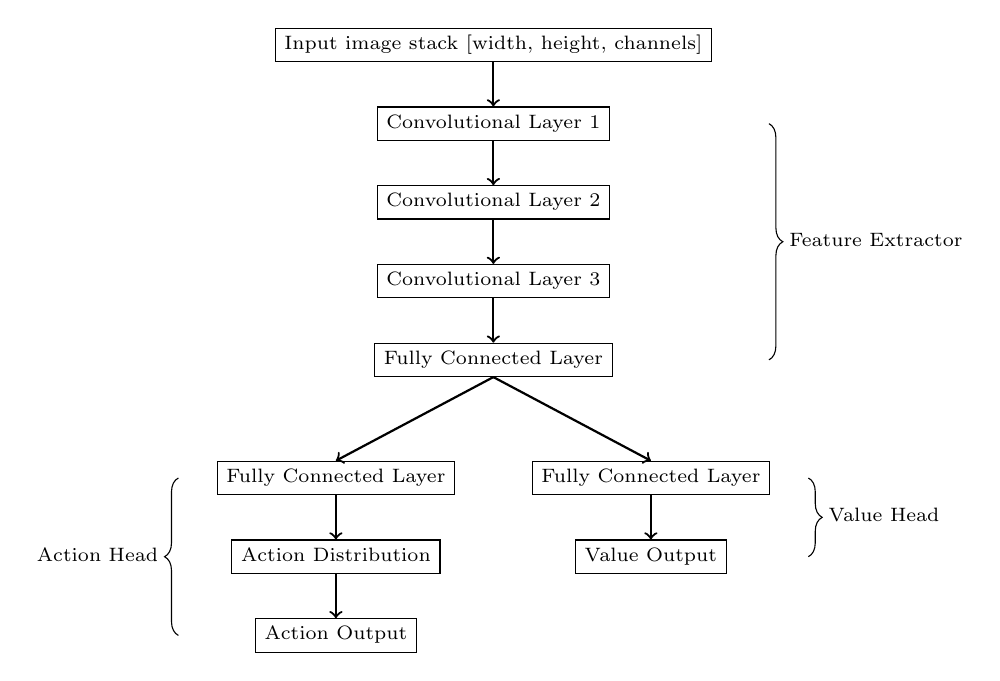
\begin{tikzpicture}[%
            every node/.style={
                    font=\scriptsize,
                    % Better alignment, see https://tex.stackexchange.com/questions/315075
                    text height=1ex,
                    text depth=.25ex,
                }, outer sep=auto
        ]

        \node[draw] (input) at (0, 0) {Input image stack [width, height, channels]};

        \node[draw] (c1) at (0, -1) {Convolutional Layer 1};
        \node[draw] (c2) at (0, -2) {Convolutional Layer 2};
        \node[draw] (c3) at (0, -3) {Convolutional Layer 3};
        \node[draw] (fc1) at (0, -4) {Fully Connected Layer};

        \draw[decorate,decoration={brace,amplitude=5pt}] (3.5,-1) -- (3.5,-4)
        node[anchor=west,midway,right=4pt] {Feature Extractor};

        \node[draw] (fcAction) at (-2, -5.5) {Fully Connected Layer};
        \node[draw] (actionDist) at (-2, -6.5) {Action Distribution};
        \node[draw] (actionOut) at (-2, -7.5) {Action Output};

        \node[draw] (fcValue) at (2, -5.5) {Fully Connected Layer};
        \node[draw] (valueOutput) at (2, -6.5) {Value Output};

        \draw[decorate,decoration={brace,mirror,amplitude=5pt}] (-4,-5.5) -- (-4,-7.5)
        node[anchor=east,midway,left=4pt] {Action Head};

        \draw[decorate,decoration={brace,amplitude=5pt}] (4,-5.5) -- (4,-6.5)
        node[anchor=west,midway,right=4pt] {Value Head};

        \draw[->,thick] (input.south) -- (c1.north);
        \draw[->,thick] (c1.south) -- (c2.north);
        \draw[->,thick] (c2.south) -- (c3.north);
        \draw[->,thick] (c3.south) -- (fc1.north);

        \draw[->,thick] (fc1.south) -- (fcAction.north);
        \draw[->,thick] (fcAction.south) -- (actionDist.north);
        \draw[->,thick] (actionDist.south) -- (actionOut.north);

        \draw[->,thick] (fc1.south) -- (fcValue.north);
        \draw[->,thick] (fcValue.south) -- (valueOutput.north);

    \end{tikzpicture}
    \caption{\ac{NN} Structure}
    \label{fig:network_structure}
\end{figure}

\subsubsection{Feature Extractor}

The feature extractor comprises the first four layers of the network. As the name suggests, the feature extractor extracts features from the input for further processing by the network.

The feature extractor consists of three convolutional layers and one fully connected layer. The first convolutional layer takes the output of the memory buffer as input. The output of the feature extractor's fully connected layer is used by the action and value heads.


\subsubsection{Action Head}
\label{sec:action_sampling}

The action head consists of a single fully connected layer with two outputs. The two outputs represent the mean of the two-dimensional action distribution. The action distribution is a Gaussian Distribution. The action distribution can be sampled deterministically or stochastically to obtain an action for the agent. The most likely action is returned in determinsitc sampling. This is equal to the outputs of the action head. In stochastic sampling, the action is sampled from the action distribution.

The sampled actions are clipped to the action space's range of $[-1,1]$. This is necessary as the sampling can return a value outside of the range.

\subsubsection{Value Head}

The value head consists of a single fully connected layer with one scalar output.


\subsection{Parameters}
The \ac{NN}'s input dimensions are determined by the agent's camera image dimensions and the observation processing. The network architecture follows the specifications from \textcite{human_level_control}. However the observation space differ from their network. This results in a different number of parameters for the feature extractor's layers.
The parameters and layer dimensions used network are shown in figure \ref{fig:network_architecture}.


% verified in code:
% action and value head share the extractor
% when sampling deterministic, the action is the mean of the distribution
% the output of the action head is the mean of the distribution

% the action head is a single linear layer, there is no activation function applied to the output

% DiagGaussianDistribution
% the log std of the distribution is a learnable parameter
% it is also updated, see policy_loss (the single parameter of size 2 that is added in the graph last)

\begin{figure}
    \begin{center}
        \begin{tabular}{|| c | p{0.25\linewidth} | p{0.4\linewidth} ||}
            \hline
            Component                          & Layer Type            & Layer Specifications                     \\ [0.5ex]
            \hline\hline
            \multirow{4}{*}{Feature Extractor} & Convolutional Layer   & 32 filters, 3 dimensional (10, 8, 8)     \\\cline{2-3}
                                               & Convolutional Layer   & 64 filters, 3 dimensional (32, 4, 4)     \\\cline{2-3}
                                               & Convolutional Layer   & 64 filters, 3 dimensional (64, 3, 3)     \\\cline{2-3}
                                               & Fully connected Layer & 512 output neurons, (512 x 12096) matrix \\
            \hline
            Action Head                        & Fully connected Layer & 2 output neurons, (2 x 512) matrix       \\
            \hline
            Value Head                         & Fully connected Layer & 1 output neuron, (1 x 512) matrix        \\
            \hline
        \end{tabular}
        \begin{tabular}{r@{: }l}
            $agentImageWidth$      & 500  \\
            $agentImageHeight$     & 168  \\
            $downsampling\_factor$ & 2    \\
            $grayscale$            & True \\
            $equalize$             & True \\
            $frame\_stacking$      & 10   \\
        \end{tabular}
    \end{center}
    \caption{\ac{NN} layers and parameters for the best configuration}
    \label{fig:network_architecture}
\end{figure}

